\section{Tracking Improvement}
\label{singleleg}


The standard CMS tracking is made of six iterative steps, numbered
from 0 to 5, designed to obtain high efficiency and low fake rate for
tracks coming either from the primary vertex or from displaced decay
vertices while maintaining the overall computing time within the
requirements of CMS offline reconstruction centre.
Because of this constraint, the standard implementation is not optimal
to reconstruct with high efficiency tracks from photon conversions and
nuclear interactions since the cuts applied in the standard
reconstruction are too tight for these processes. In fact, those
tracks have usually very low momentum and, especially for displaced
vertices at large radii, they do not point  back to the primary
vertex; therefore, they could be reconstructed only with very relaxed
cuts that would result into unacceptably large computing time during
the pattern recognition.

For the purpose of the present study, two additional dedicated
tracking steps are added to the track reconstruction sequence.
These were specifically designed to increase the number of
reconstructed conversion vertices in the barrel region,
but they have been found to be very useful for nuclear interaction as
well. A first additional step (step 6) is seeded from triplets of hits
in the Pixel barrel and/or in the Strip Tracker Inner barrel
detectors; a second additional step (step 7) is seeded from hit-pairs
in the Strip Tracker barrel detectors and/or in the Strip Tracker Inner disks.
The seed trajectories are required
%to originate from a region of radius $25\cm$ and longitudinal half length of $0.5\cm$ and are required                                                                                            
to have a minimum transverse momentum of $0.1$ and $0.2\GeVc$ for the
step 6 and 7, respectively. The resulting large number of seeds is
reduced by selecting topologies compatible with a photon conversion
pair: the total charge has to be zero,
the azimuthal angle difference less than $1.5$ radians, the difference
in the cotangent of the polar angle less than $0.25$ radians, and the
differences of the radial and longitudinal coordinates of the
innermost hit have to be less then $5\cm$.
The pattern recognition is then performed allowing for at most one
lost hit and requiring at least three hits. Finally the standard track
fit provides the best estimate of the track parameters.

The impact of the additional steps to the reconstruction of conversion
and nuclear interaction vertices can be seen on Fig.~\ref{fig:matItTk}
showing the contribution of the different steps to the vertices
reconstruction, as estimated by the simulation.
Step 7 increases by more than a factor two the number of conversions
outside the Pixel detector region and contributes significantly to nuclear
interaction vertices at all radii; step 6 mainly helps finding
conversions in the second and third Pixel detector layers. Further details
about the reconstruction of conversions and nuclear interactions will
be given in the following sections.
\begin{figure}[!hbtp]
\centering
\subfigure[]{
\label{subfig:convItTk}
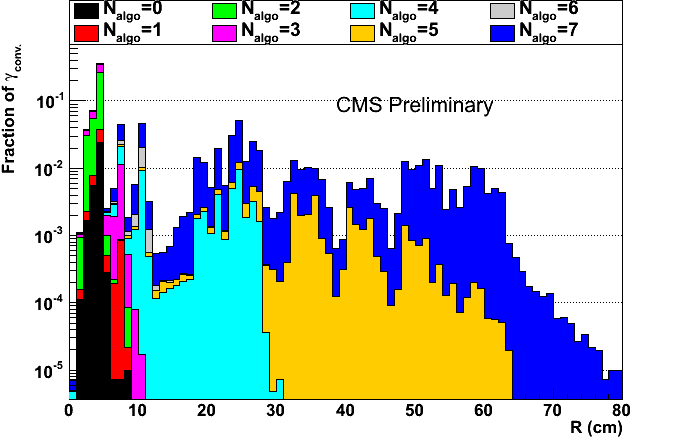
\includegraphics[width=.7\textwidth]{fig/r_algo_BasicCutsJuly12.png}}
\subfigure[]{
\label{subfig:nuclItTk}
\includegraphics[width=.7\textwidth]{fig/r_algo_2010-06-04_NI.png}}
\caption{Fraction of reconstructed vertices as a function of the radius of the vertex
for conversions~\subref{subfig:convItTk} and nuclear
interactions~\subref{subfig:nuclItTk}, for  $|\eta|<1.4$, as estimated
from simulation. The different colors correspond to the largest
iterative step needed to reconstruct the tracks at the vertex.}
\label{fig:matItTk}
\end{figure}
